% Compile with: lualatex mandelbrot.tex
\documentclass[11pt]{article}

\usepackage{amsmath, amssymb}
\usepackage{tikz}
\usepackage[a4paper, margin=2.5cm]{geometry}
\usepackage[colorlinks=true, urlcolor=blue]{hyperref}
\usepackage{fancyhdr}

\pagestyle{fancy}
\fancyhf{}
\renewcommand{\headrulewidth}{0pt}
\fancyfoot[L]{\small Junzhe Wang ~\textperiodcentered~
  \href{mailto:junzhe.wang2002@gmail.com}{\texttt{junzhe.wang2002@gmail.com}}}
\fancyfoot[R]{\small Last edited: \today\ ~\textperiodcentered~ p.\,\thepage}

\title{The Mandelbrot Set}
\author{}
\date{}

\begin{document}

\maketitle
\thispagestyle{fancy}

\section{Definition}

Fix a point $c = (a, b)$ of the plane, viewed as the complex number
$c = a + ib$, and iterate the map
\begin{equation}
  z_0 = 0, \qquad z_{n+1} = z_n^2 + c.
\end{equation}
The \emph{Mandelbrot set} $M$ is the set of parameters $c$ for which this
sequence remains bounded. Writing $z_n = x_n + i y_n$ and separating real and
imaginary parts gives the purely real recurrence used by the program:
\begin{equation}
  x_0 = y_0 = 0, \qquad
  \begin{cases}
    x_{n+1} = x_n^2 - y_n^2 + a \\
    y_{n+1} = 2 x_n y_n + b.
  \end{cases}
\end{equation}

\section{The escape criterion}

Membership asks about the sequence's behavior at infinity, which no finite
computation can decide directly. Two facts rescue the programmer:
\begin{enumerate}
  \item If $|z_n| > 2$ for some $n$, the sequence diverges. Indeed, once
    $|z| > 2$ and $|z| \geq |c|$,
    \[
      |z^2 + c| \;\geq\; |z|^2 - |c| \;\geq\; |z|^2 - |z|
      \;=\; |z|\,(|z| - 1) \;>\; |z|,
    \]
    and the modulus grows at an accelerating rate thereafter. Consequently
    $M$ is contained in the closed disk of radius $2$, and the program's test
    $x_n^2 + y_n^2 > 4$ is a sound divergence certificate.
  \item In practice, points outside $M$ tend to escape quickly, so testing the
    first $k$ terms (the book uses $k = 100$) classifies all but a thin sliver
    near the boundary correctly.
\end{enumerate}

The \emph{escape time} of a point $c \notin M$ is the first index $n$ with
$|z_n| > 2$. It measures how close $c$ is to the set --- distant points escape
in a handful of steps, points hugging the boundary may take hundreds --- and
coloring pixels by escape time produces the familiar glowing halos around the
fractal.

\begin{center}
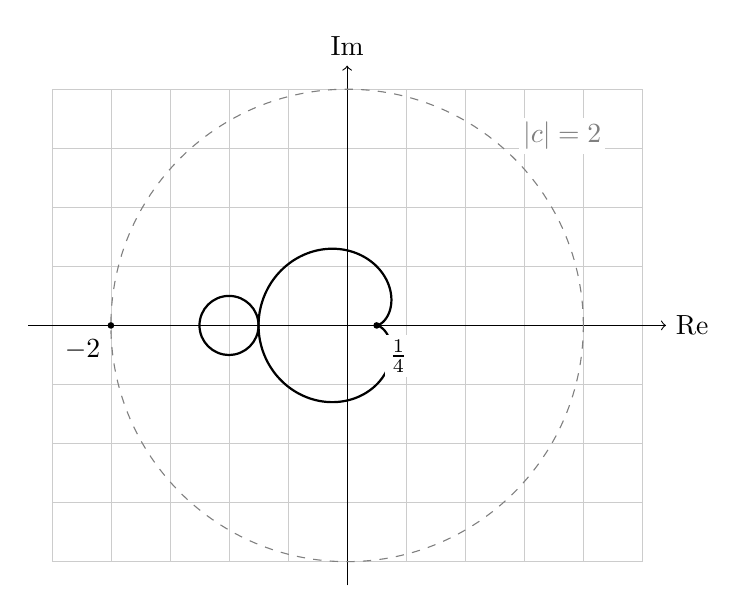
\begin{tikzpicture}[scale=1.5]
  \draw[very thin, gray!40] (-2.5, -2) grid[step=0.5] (2.5, 2);
  \draw[->] (-2.7, 0) -- (2.7, 0) node[right] {$\mathrm{Re}$};
  \draw[->] (0, -2.2) -- (0, 2.2) node[above] {$\mathrm{Im}$};
  % escape disk of radius 2
  \draw[dashed, gray] (0, 0) circle (2);
  \node[gray, fill=white, inner sep=1.5pt, above right] at (1.45, 1.45)
    {$|c| = 2$};
  % main cardioid: c = e^{it}/2 - e^{2it}/4
  \draw[thick, domain=0:360, samples=400, smooth]
    plot ({cos(\x)/2 - cos(2*\x)/4}, {sin(\x)/2 - sin(2*\x)/4});
  % period-2 disk
  \draw[thick] (-1, 0) circle (0.25);
  \fill (0.25, 0) circle (0.8pt);
  \node[fill=white, inner sep=1.5pt, below right] at (0.32, -0.08) {$\tfrac14$};
  \fill (-2, 0) circle (0.8pt);
  \node[fill=white, inner sep=1.5pt, below left] at (-2.05, -0.08) {$-2$};
\end{tikzpicture}

\smallskip
The two largest pieces of $M$: the main cardioid and the period-2 disk,
inside the escape disk $|c| \leq 2$.
\end{center}

\section{Properties}

\begin{itemize}
  \item \textbf{A cardioid again.} The big heart-shaped body of $M$ is an
    exact cardioid: the parameters $c = \frac{e^{i\theta}}{2} -
    \frac{e^{2i\theta}}{4}$ for which the iteration has an attracting fixed
    point. Our previous quiz drew its cousin.
  \item \textbf{Bounded but intricate.} $M$ fits in the disk of radius 2, is
    connected (Douady--Hubbard, 1982), and its boundary is so wrinkled that
    its Hausdorff dimension is 2 (Shishikura, 1998).
  \item \textbf{On the real line.} $M \cap \mathbb{R} = [-2, \tfrac14]$: the
    program's test points $(0,0)$, $(-1,0)$, $(-2,0)$ are members, while
    $(1, 0)$ escapes in three steps.
  \item \textbf{Self-similarity.} Zooming anywhere near the boundary reveals
    miniature copies of the whole set --- the hallmark of a fractal.
\end{itemize}

\section{From mathematics to pixels}

The program scans every pixel $(w, h)$ of the window, maps it affinely to a
point $(a, b) \in [-2, 2]^2$, and iterates the recurrence at most $k$ times.
If $x_n^2 + y_n^2$ never exceeds $4$, the pixel is considered a member and
plotted. The precision of the picture depends only on $k$: raising it sharpens
the boundary at the price of more arithmetic on the points that never escape.

\end{document}
